\documentclass[letterpaper, 10pt]{article}
\usepackage[OE]{express}
\usepackage{multirow}
\usepackage{graphicx}
\usepackage{subfigure}
\usepackage{cite}
\usepackage{soul}

\begin{document}
\title{Silica-based integrated 1$\times$4 polarization beam splitter module for free-space BB84 quantum key distribution}
\author{Joong-Seon Choe, Heasin Ko, Byung-Seok Choi, Kap-Joong Kim, and Chun Ju Youn}
\address{Electronics and Telecommunications Research Institute, Daejeon 34129, Korea}
\email{jschoe@etri.re.kr}

\begin{abstract}
We have developed an integrated polarization beam splitter (PBS) module with silica planar lightwave circuit technology for use in BB84 quantum key distribution (QKD).
The PBS module was designed to operate on four linear polarizations of horizontal/vertical/diagonal/antidiagonal direction, and showed the minimum polarization extinction ratio of 17.6 dB.
When the module was loaded on the free-space BB84 QKD test-bed, quantum bit error rate and sifted key rate  were 2.81\% and 415 kbps at clock rate of 100 MHz, respectively.
\end{abstract}

\ocis{(260.5430) Polarization; (230.5440)   Polarization-selective devices; (060.5565) Quantum Communications; (230.7390) Waveguides, planar }

\bibliographystyle{osajnl}
% \begin{thebibliography}{1}
% \newcommand{\enquote}[1]{``#1''}
% \expandafter\ifx\csname url\endcsname\relax
%   \def\url#1{\texttt{#1}}\fi
% \expandafter\ifx\csname urlprefix\endcsname\relax\def\urlprefix{URL }\fi
% \providecommand{\eprint}[2][]{\url{#2}}

\bibliography{jschoe}
% \end{thebibliography}

\section{Introduction}

Many researches have been conducted for quantum communication as security solution is one of the main issues in communication technology \cite{Bennett:1984is, Ekert:1991kl,Ko:2017cs}.
Since Bennett and Brassard proposed BB84 protocol for secure key distribution, it has widely been chosen for quantum key distribution (QKD) \cite{Bennett:1984is}.
Implementation of BB84 requires two sets of non-orthogonal basis
that are usually constructed with polarization of single photon for free-space communication.
The polarization-based BB84 protocol encodes the data by choosing a basis of the two bases of horizontal(H)/vertical(V) or diagonal(D)/antidiagonal(A) polarization, and transmitting a single photon of a polarization from the chosen basis to generate an encryption key.

Thus an optical part for splitting or combining the four states of polarization is essential for a polarization-based BB84 QKD, and is generally composed of two bulk polarization beam splitters (PBS), one beam splitter, and one half-wave plate (HWP) \cite{Ko:2017cs}.
Although the bulk-optic components show high performances in polarization extinction ratio (PER), optical loss, and so on, the QKD system will work only when the components are installed with high alignment accuracy upon which its overall performance is strongly dependent.


The need for alignment of discrete optic components can be removed if they are replaced by  a passive photonic chip with integrated elements
fabricated through semiconductor processes such as photo-lithography and dry etching.
The chip-scale integration of the optical part of BB84 system provides miniaturization necessary to diversify application area such as QKD for hand-held devices, and makes it possible to achieve mass production with low cost.
In view of performance, the integration improves stability of QKD system because optical transmission characteristics of a passive photonic chip is quite stable.
PBS chips using waveguide are widely used in optical receivers for polarization-multiplexed modulation formats such as dual polarization quadrature phase shift keying (DP-QPSK), dual polarization 16 quadrature amplitude modulation (DP-16QAM), etc  \cite{Lee:2016bg,PoDong:2014kj}.
However, there has been no report on integrated PBS chip that can deal with four polarizations used in BB84 QKD.
In this study, integrated PBS module using  silica-based planar lightwave circuit (PLC) chip was fabricated for the first time for BB84 protocol, and its performance was assessed it in a free-space QKD test-bed.

\section{Fabrication}
\subsection{PBS chip}


PBS developed in this work is based on Mach-Zehnder interferometer (MZI) structure fabricated with silica PLC technology, as is shown in Fig. \ref{fig:layout}(a)\cite{Kim:2012ej, Hashizume:2015ta}.
The waveguide structure was chosen to support single mode and maximum mode matching with single mode fiber (SMF) at the operating wavelength of 780 nm, where Si-based single photon detector has high detection efficiency and atmospheric absorption is low.
Refractive indices of core and clad material were 1.4588 and 1.4537 at 780 nm, respectively, and the dimension of the waveguide core was designed as 4.3 $\mu$m $\times$ 4.3 $\mu$m.

In Fig. \ref{fig:layout}(a), the input light is split into two paths by a 3 dB splitter.
At the outputs of the splitter are connected in parallel two identical MZIs with 2$\times$2 multimode interference (MMI) coupler.
A portion of the waveguide of upper arm in each MZI was designed to have larger width of 18.5 $\mu$m.
A wide waveguide in silica PLC is known to have birefringence  due to uniaxial strain generated in the fabrication process \cite{Okuno:1994fm}.
The birefringence causes relative phase differences between H- and V-polarized lights when light reaches the  input of the MMI through the arms.
When the device is designed so that birefringence $\Delta n$ and length $L$ of the wide waveguide satisfy the condition $2\pi\Delta n/\lambda  = (2m+1) \pi$ with integer $m$, the phase difference between H- and V-polarization can be made to be 180$^\circ$.
If above condition is satisfied and the lower arm is made to provide a phase difference of 90$^\circ$ between the arms for the two polarizations, polarization separation is achieved according to the operation of MMI depicted in Fig. \ref{fig:layout}(b).


The phase relationship is determined by arm length, as described above.
But actually it changes sensitively with ambient temperature around the interferometer structure.
Therefore, micro-heaters were deposited on the arms of MZI to actively control the phase making use of the thermo-optic property of silica.

The input light may be in D/A-polarization basis as well as H/V-polarization basis, but D- and A-polarized light can not be properly separated in PLC PBS composed of rectangular waveguide.
In this study, a HWP film with its optic axis tilted by 22.5$^\circ$ was inserted at the input of the lower PBS to split D/A polarization.
Although the output of the lower MZI is annotated as D/A in Fig. \ref{fig:layout}, actual polarization of the output light is H/V.

\begin{figure}
  \centering
  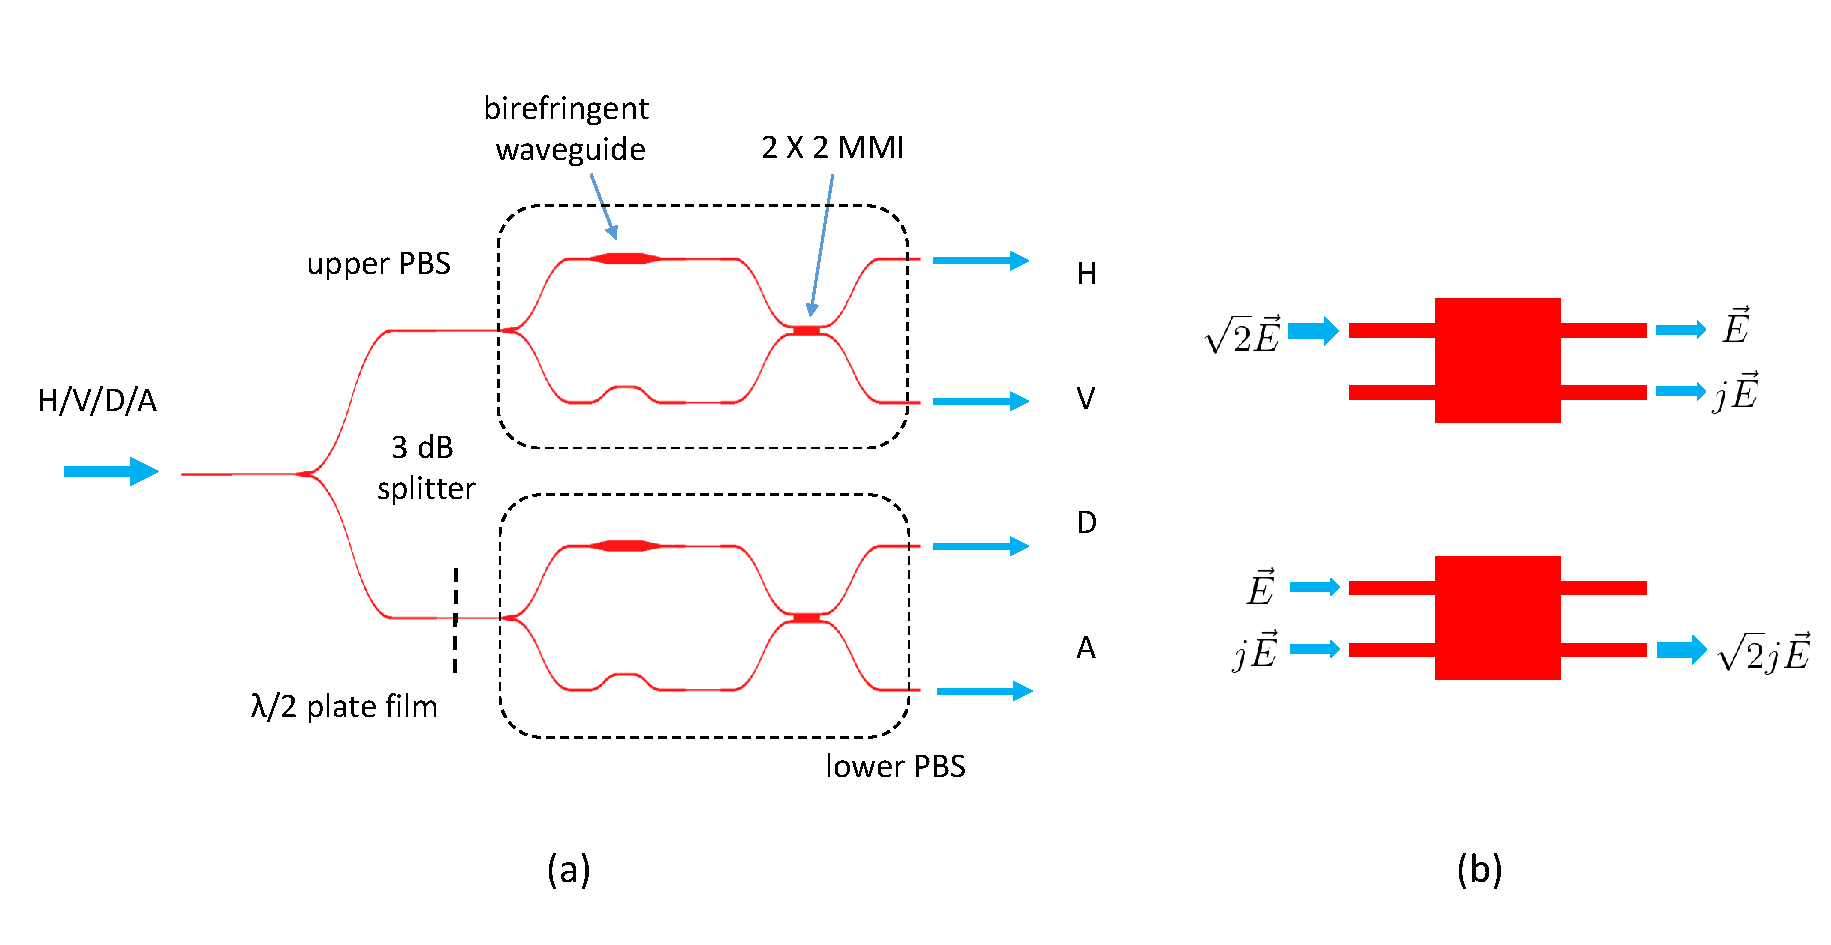
\includegraphics[height=6.3cm]{./layout}
  \caption{(a) Layout of the PBS device for H/V/D/A-polarizations. 1$\times$2 splitter splits the input light into two PBSes that separate H- and V-polarization and output them to the corresponding waveguides. Lower PBS has HWP at its input so that D- or A-polarized light is converted to H- or V-polarization. (b) Schematic description of the operation of 2$\times$2 MMI. Under single port input, the two outputs show electric field with same amplitude and relative phase difference of 90$^\circ$ (upper). If there is phase difference of 90$^\circ$ between two input electric fields, one output is extinguished (lower).}
  \label{fig:layout}
\end{figure}


\subsection{Half-Wave Plate Film}

Thin film HWP was developed for converting D/A polarization to H/V polarization that can be inserted in a slit across a waveguide.
A HWP was fabricated by imposing birefringence on a polymer film \cite{Ando:1993up}.
Fixed at its two sides on a metal frame designed for elongation process, the film was stretched at an elevated temperature.
Elongation process was performed for several kinds of commercial polymer film under various conditions, and it was found that 40\% elongation of 60-$\mu$m-thick polycarbonate film at 170$^\circ$C resulted in retardance near 180$^\circ$ at the wavelength of 780 $\mu$m.
The thickness of the film after process was 53 $\mu$m.
As the film was to be used for light of D/A polarization, cutting direction was selected so that the optic axis was inclined by 22.5$^\circ$ with respect to the bottom side of the film.

\subsection{PBS Module}

Firstly, a narrow groove was formed at the input waveguides of two parallel MZIs comprising 1$\times$4 PBS with a dicing blade for the insertion of the waveplate film.
Waveplate is needed for only one MZI of the PBS, but the groove spans  both the MZIs because of the small separation of 500 $\mu$m, resulting in similar optical loss between the two MZIs.
When processed with 50-$\mu$m-thick blade, the width of the groove formed was about 62 $\mu$m.
After the waveplate film was inserted into the groove, UV-cured epoxy was injected to fix it.

Pigtailed were an SMF on the input facet and 4-channel polarization-maintaining fiber (PMF) array on the output facet.
Both the PBS chip and fibers were angle (8$^\circ$)-polished to reduce the optical return loss that influences the stable operation of LD.
The four PMFs were aligned so that the slow-axes  were oriented alternately as H-V-H-V.
Using this PMF array, the module can be used as polarization beam combiner (PBC) as well as PBS.

The pigtailed chip was mounted in a module housing with a thermoelectric cooler (TEC) and a thermistor pre-installed.
Wire-bonding of the heater of MZIs finalized the module assembly procedure.
Figure \ref{fig:module} shows the fabricated module mounted on a control-board.
\begin{figure}
  \centering
  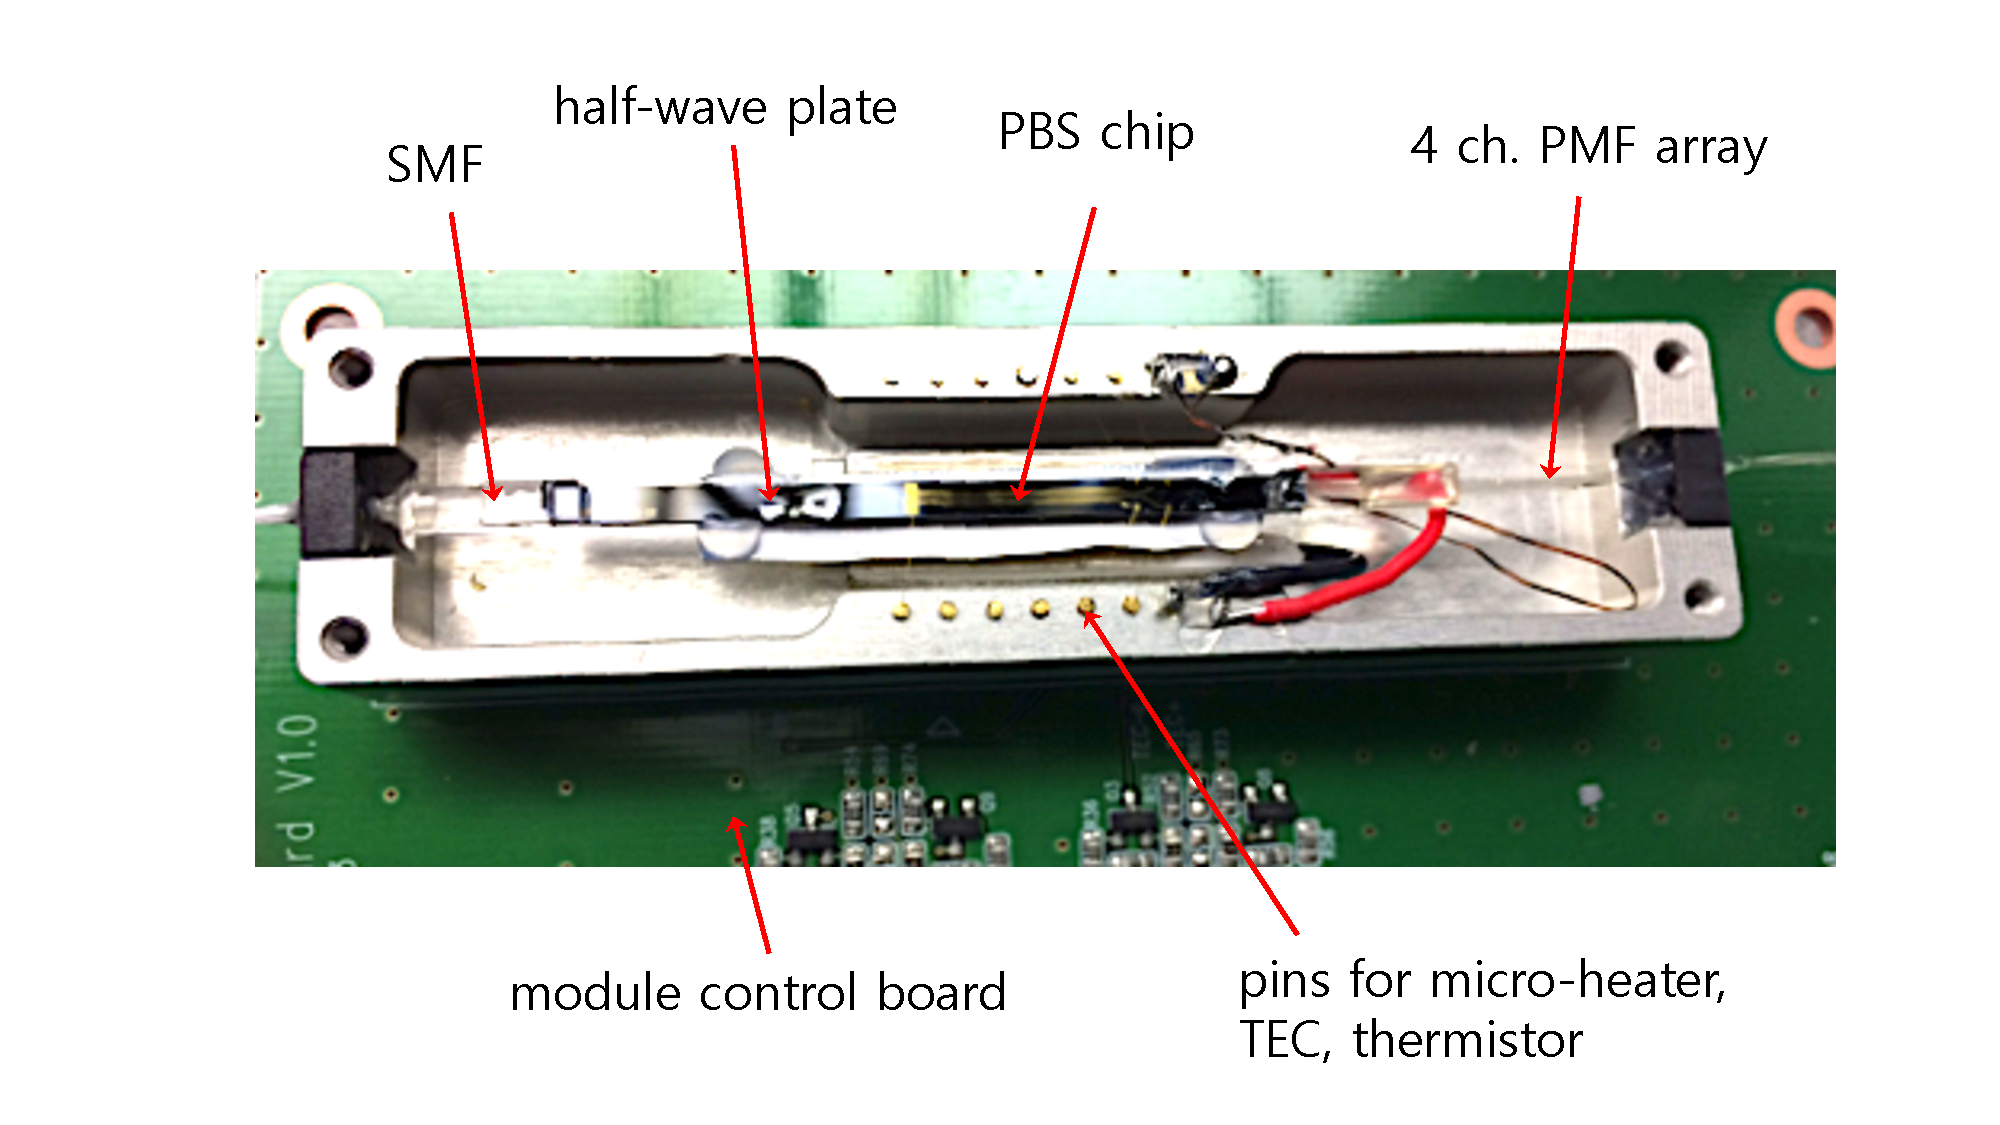
\includegraphics[height=6cm]{module.pdf}
  \caption{PBS module consists of PBS chip with inserted HWP, TEC, thermistor, SMF, and PMF array. Micro-heaters of the PBS chip were wire-bonded to the pins of the module housing. The module is mounted on a board that controls chip temperature and currents of the micro-heater.}
  \label{fig:module}
\end{figure}

\section{Characterization}
\subsection{PBS chip}

Measurement setup of Fig. \ref{fig:setup}  was used to characterize the polarization splitting property of the PBS chip.
\begin{figure}
  \centering
  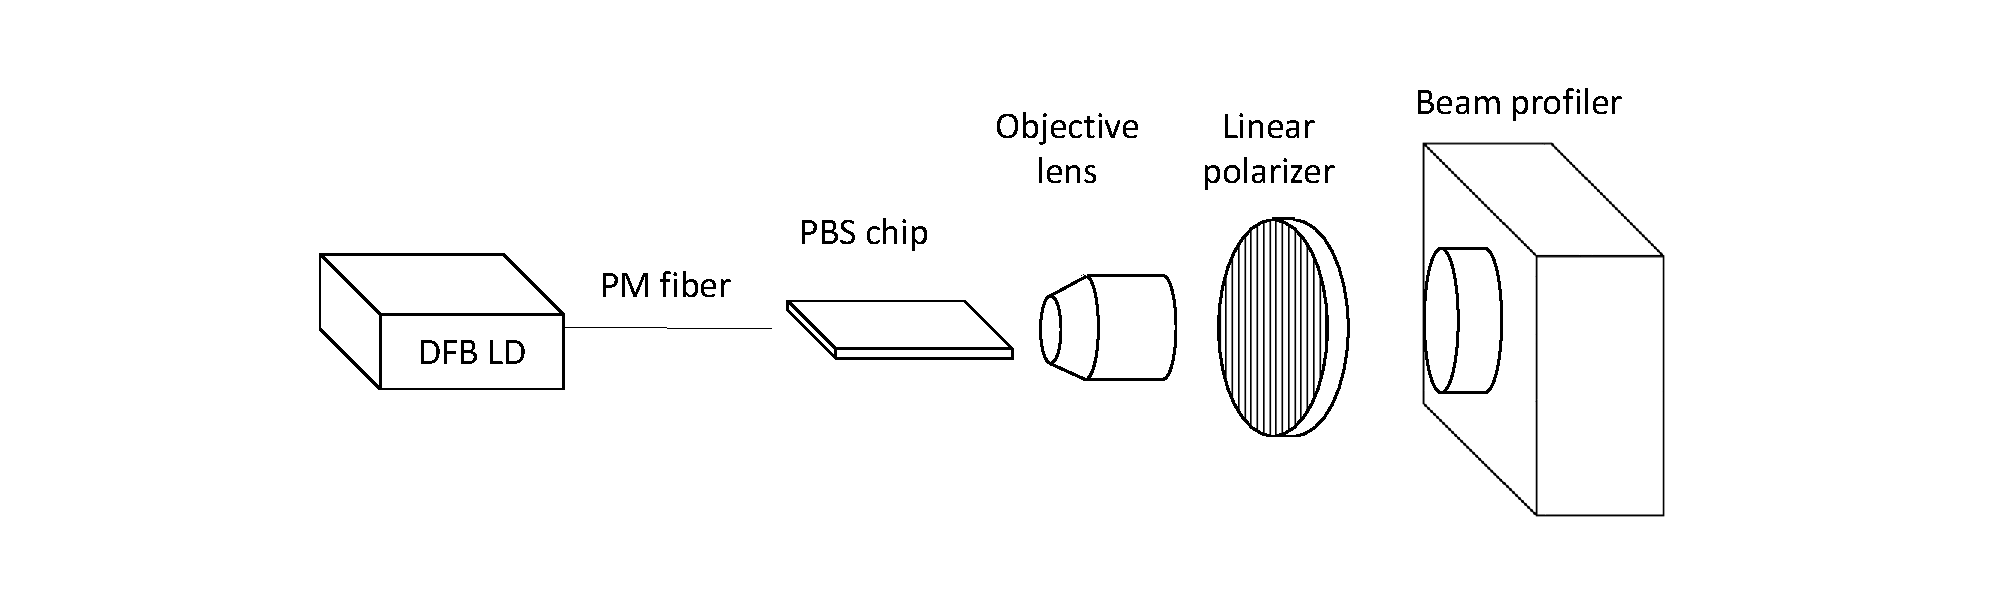
\includegraphics[width=13cm]{./setup.pdf}
  \caption{Schematic of the setup measuring PER of PBS chip. Obliquely polarized light is incident on the chip via PMF. The linear polarizer filters out the transmitted light to either H- or V-polarization, and the beam profiler measures the output power ratio of each waveguide.}
  \label{fig:setup}
\end{figure}
Output of a 780 nm distributed fee dBack LD was delivered to the PBS chip through a polarization-maintaining fiber (PMF) whose slow axis is aligned obliquely so that incident light contains both H- and V-polarization.
The output light from the chip was expanded through an objective lens and observed using a beam profiler (Ophir Optronics Spiricon SP503).
As the input polarization is neither H nor V, output light has both the polarizations.
In order to evaluate polarization extinction ratio (PER), a linear polarizer (LP) was placed between the objective lens and beam profiler.
If the transmission axis of the LP is vertical, only V-polarized light is considered to be incident on the beam profiler since the LP filters out the H-polarized light with high PER exceeding 30 dB.
This method is based on the assumption that rotation of polarization does not occur for both H- and V-polarized lights.
With polarization rotation in the PBS chip, PER would be deteriorated when measured after the chip is fabricated to PBS module that does not contain LP.
As will be discussed later, however, PBS module does not show any drop of PER, which suggests the validity of the assumption.

PER was obtained by measuring the intensity from the output waveguides using a beam profiler while the current of the micro-heater was adjusted so that PER of PBS could be maximized.

The PBS chip showed different PER characteristics depending on the length of the birefringent waveguide (BRW) as shown in Fig. \ref{fig:BRW-PER}.
\begin{figure}
  \centering
  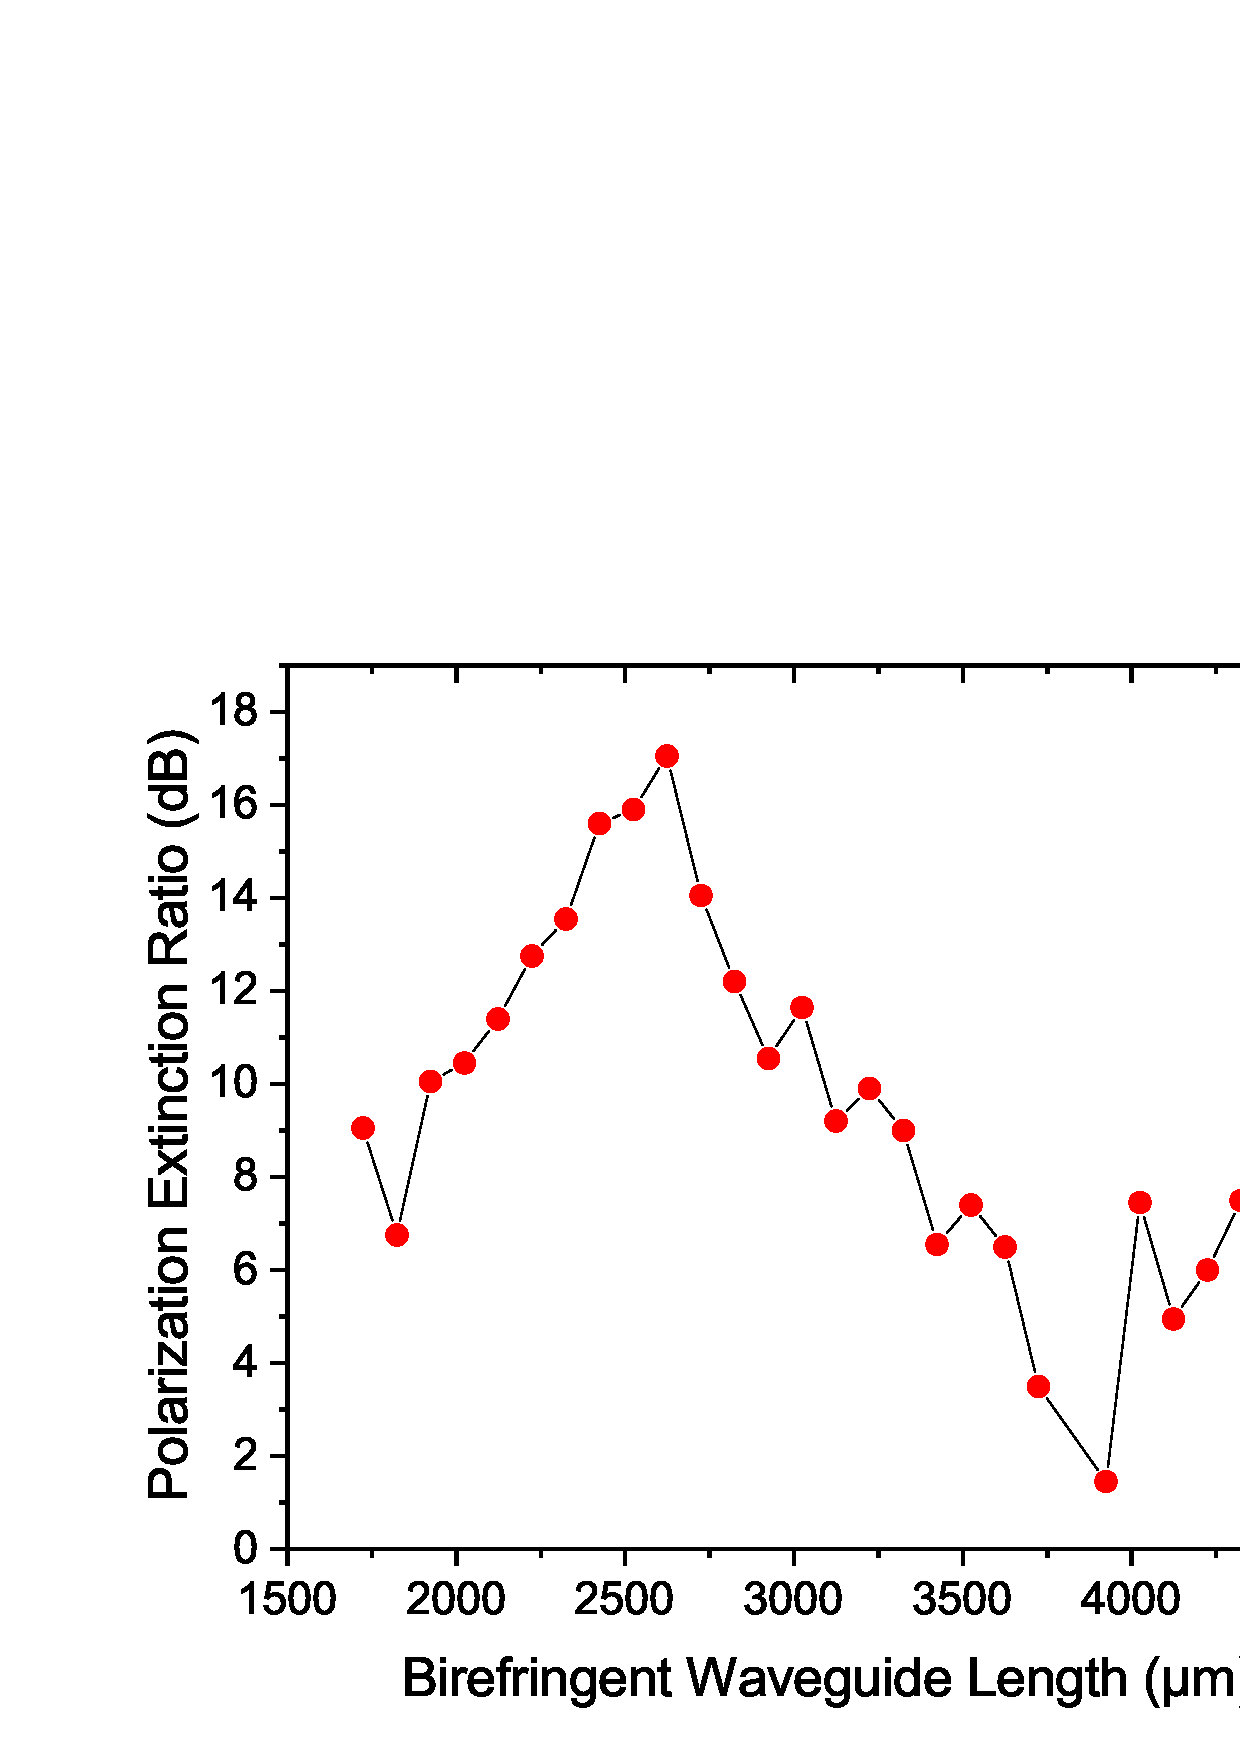
\includegraphics[width=7cm]{./BRWPER.pdf}
  \caption{Measured result of PER with birefringent waveguide length. Maximum PER of 17.1 dB was obtained when the BRW length is 2624 $\mu$m.}
  \label{fig:BRW-PER}
\end{figure}
Maximum PER was measured as 17.1 dB  when the length of BRW was 2624 $\mu$m.
From this result, the birefringence of the BRW is estimated as 1.5$\times 10^{-4}$ that is similar to that reported in Ref. \cite{Hashizume:2015ta}.


\subsection{Half-Wave Plate Film}
The optical output of the LD  was collimated and converted to D-polarized light by using a linear polarizer, and was transmitted through the waveplate film.
The resultant polarization state of the light was measured using a polarimeter (Thorlabs PAX5720IR1).
While the film exhibited spatial variation in retardance and direction of the optical axis, some areas of the film were measured to be suitable for use in PBS.
Part of the film converting D(A)-polarization to H(V)-polarization was cut out into a size of 1.5 mm $\times$ 1.0 mm for being inserted into the groove of the PBS chip.

The direction of the optic axis may have a slight offset after the cutting  or  insertion process.
Figure \ref{fig:angle_offset} shows how PER is affected by the offset angle from 22.5$^\circ$.
\begin{figure}
  \centering
  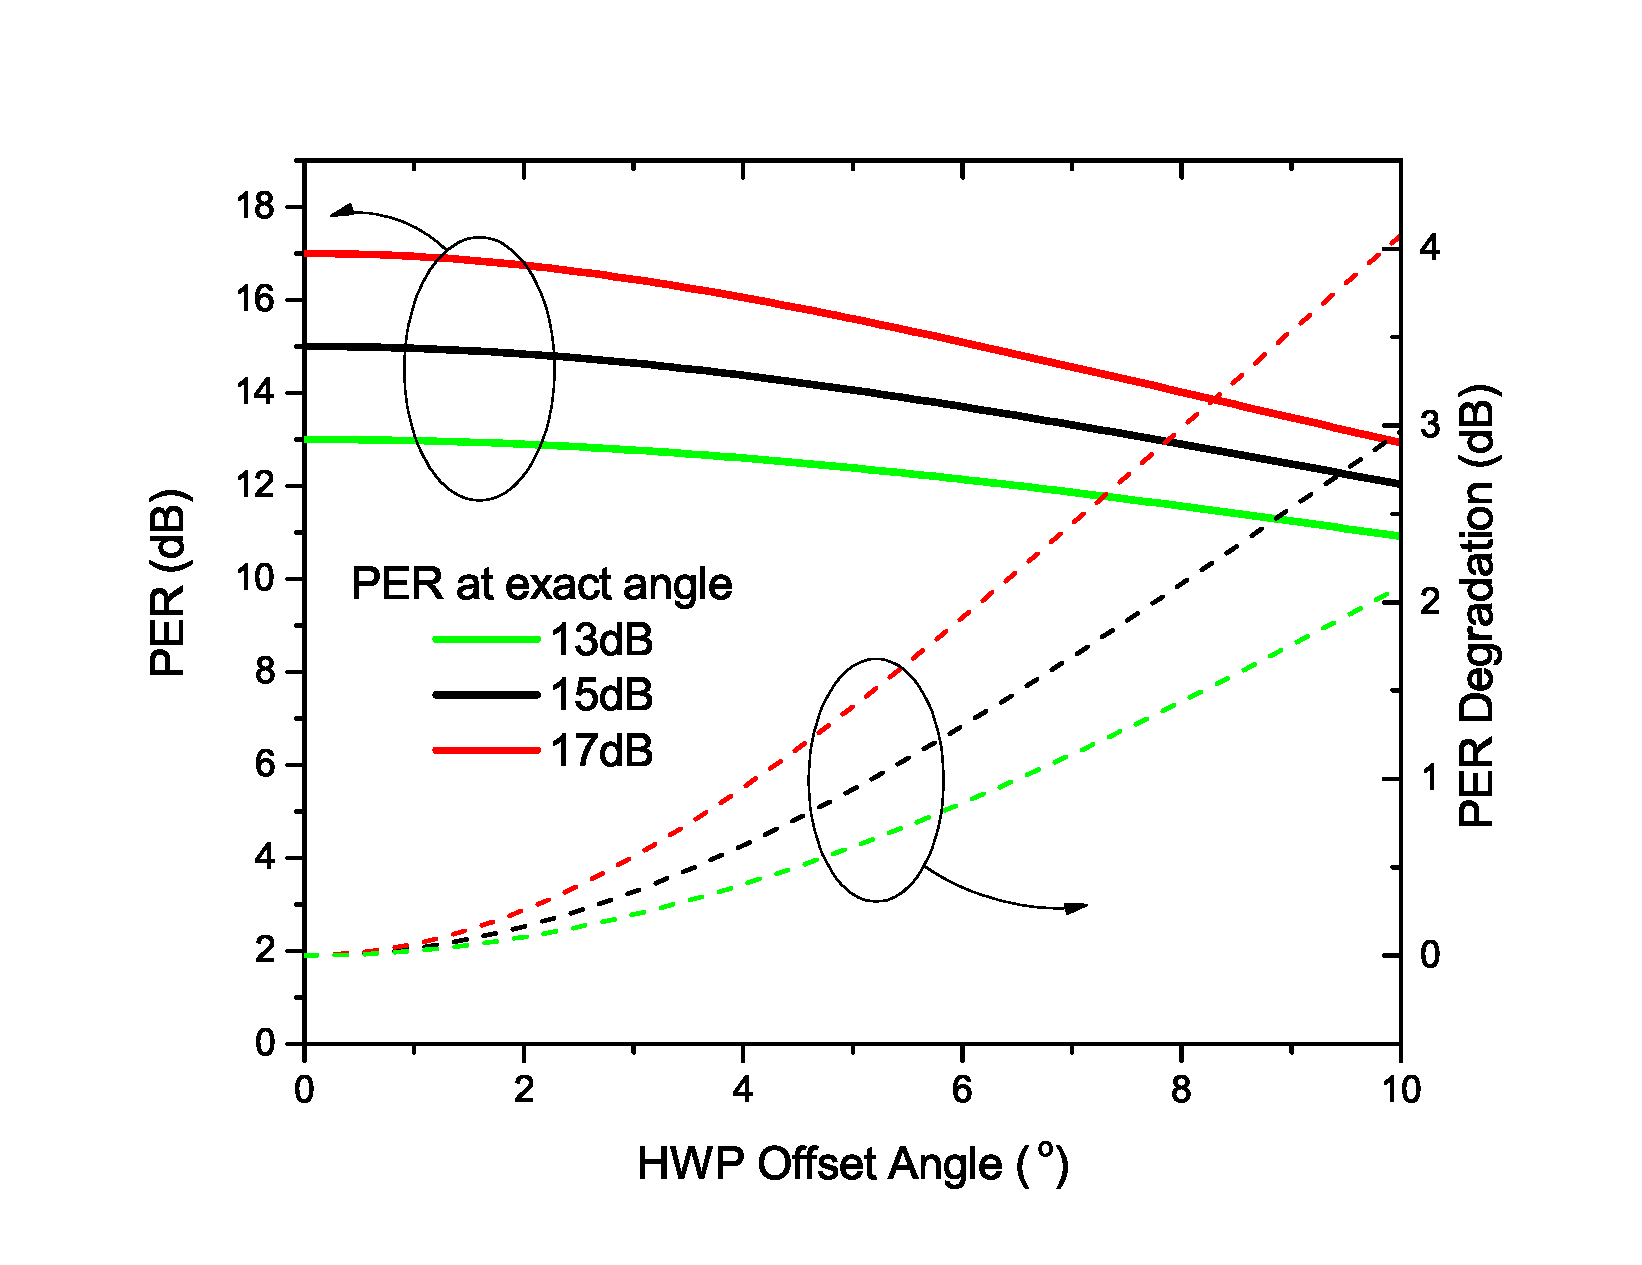
\includegraphics[width=8cm]{./offset_angle}
  \caption{PER (left axis) and its degradation (right axis) as functions of the offset angle of HWP inserted in PBS for DA-polarization. PER decreases with the offset angle, and the degradation is the larger when PER at exact angle is the higher.}
  \label{fig:angle_offset}
\end{figure}
PER gets degraded with the increase of the offset angle.
The offset angle prevents the 45$^\circ$ polarized incident light from being converted into purely V-or H-polarized light, thus reducing PER of the PBS behind the HWP.
However, Fig. \ref{fig:angle_offset} suggests that the drop of PER is not so large within  offset angle of 2$^\circ$, and  a slight angle inaccuracy does not significantly affect the overall performance.
In our study, the film cutting or treatment could be accomplished without any specialized equipment within that precision.

\subsection{PBS Module}

The polarization-splitting characteristics of the module were evaluated by receiving light from sender (Alice) of free-space QKD test-bed and measuring the optical powers from the four PMFs of the PBS module, as shown in Fig. \ref{fig:meas_setup}(a).
At the chip temperature of 21$^\circ$C and current of the micro-heater of 29 mA, the module shows PER of 22.4 dB in separating H/V polarizations, and 17.6 dB for D/A polarizations.
This is better than the result obtained from PBS chip measurement.
It is owing to both temperature optimization and better fiber-chip alignment in the module.
In chip measurement, it is difficult to align fiber with right angle to the facet of the chip.
Therefore stray light transmitted through outside of the waveguide can be coupled to unwanted output path and decrease PER of PBS.
On the other hand, the V-groove block for fiber-pigtail in module fabrication helps normal incidence of light and thus minimizes stray light.

While this polarization-splitting capability is used before single-photon detectors by receiver (Bob), the module can also be used as PBC for combining four polarization states by Alice.
Since common SMF is used as the output port in the module, there is no need to perform precise alignment so that the four polarized lights propagate along the identical path in the free space.

If four PMF-pigtailed LDs are connected to the PMFs of the PBS module, output polarizations of the LDs are converted to H-V-H-V  by the PMFs of the module, and converted to  H-V-D-A  by the HWP film in the PBS chip.

The performance of the module as a PBC was assessed by connecting the SMF of the module with a polarimeter via a polarization controller (PC) that is configured to compensate the polarization distortion occurring in the SMF, as shown in Fig. \ref{fig:meas_setup}(b).
If the module is not properly fabricated, no configuration of the PC can recover the four LDs' output to their original states simultaneously.
The four states of the polarization measured are shown in Fig. \ref{fig:meas_setup}(c).
\begin{figure}
  \centering
  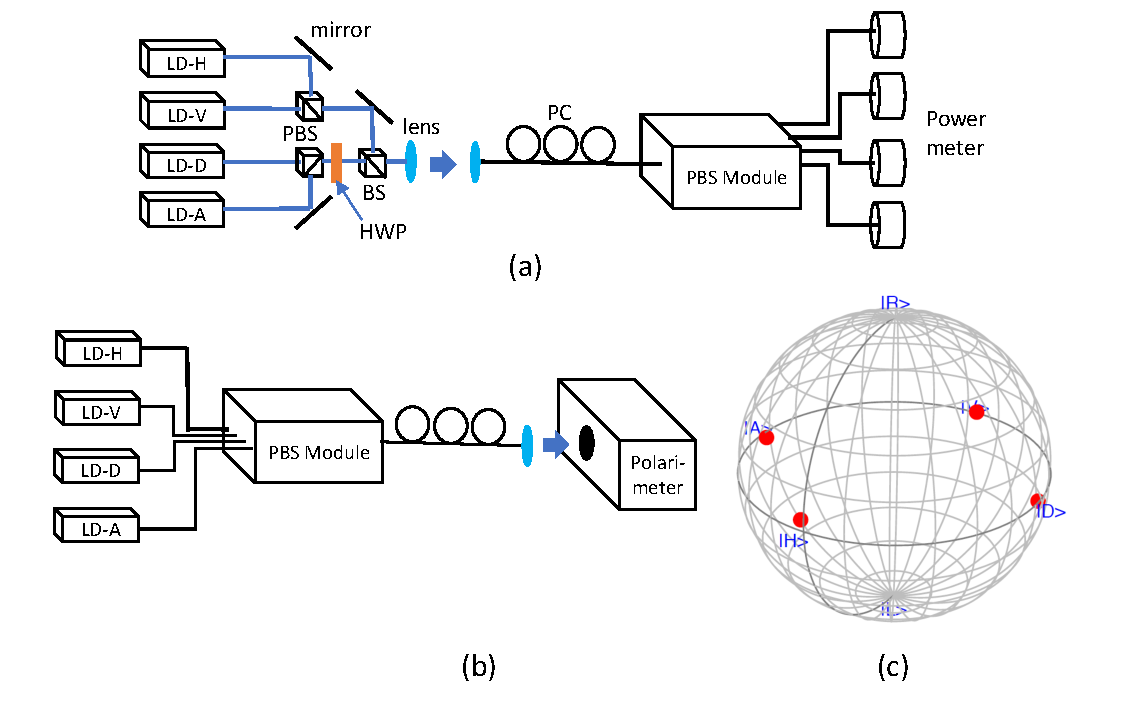
\includegraphics[height=7.5cm]{meas_setup}
  \caption{(a) Setup for measuring PER of the PBS module using Alice part of a free-space QKD test-bed. PBS module splits the input light according to its polarization, and power ratio between the outputs are obtained by measured optical powers.  (b) Setup for characterizing the module as a PBC. Output from the four LDs are combined in the module and emitted through the SMF. PC is configured to compensates all the polarization. The final polarization state  is observed by the polarimeter. (c) Measured polarization states of the module output when used as a PBC.}
  \label{fig:meas_setup}
\end{figure}
Each output state is quite close to the four polarization states of H/V/D/A.
The minimum extinction ratio of the output was as large as 346:1.
The good performance of the module as a PBC suggests the exact retardance and optic-axis alignment of the HWP film.



Total optical  loss of the module was measured to be 7.7 dB including 3 dB splitting loss of Y-branch.
The fiber-chip coupling loss at both the facets was estimated to be 1.0 dB from additional experiment.
Therefore excess optical loss occurring in the chip is about 3.7 dB.
This loss is mainly due to the groove for HWP film insertion.
Diffraction loss occurs at the waveguide gap caused by the groove, and it increases drastically with increasing gap width \cite{Inoue:1997es}.
Chipping that might occur on the edge of the diced groove surface can cause scattering loss \cite{Carpenter:2013fh}.

It is expected from a beam propagation method simulation that the loss will be decreased by about 1.5 dB if the width of the groove is reduced to 30 $\mu$m by developing thinner half-wave plate film.
The loss can be further reduced if groove-dicing process is optimized to suppress chipping.

\subsection{QKD Test}

The free-space BB84 test was performed with the fabricated module replacing the four polarization splitting block on the Bob's part of the test-bed, as shown in Fig. \ref{fig:testbed}.
\begin{figure}
  \centering
  \includegraphics[width=13cm]{testbed3.pdf}
  \caption{Setup for evaluating the integrated PBS module in the Bob part of a free-space QKD system. The module replaced one BS, one HWP, and two PBSes. Attn.: attenuator, DM: dichroic mirror, Sync. Laser: synchronization laser, M: mirror, Sync. Detector: synchronization detector, PC: polarization controller, SPD: single photon detector, FPGA: field-programmable gate array}
  \label{fig:testbed}
\end{figure}
In the Alice's part, two random number generators were used to choose the basis and binary data, and one of the four LDs emitted light accordingly at the clock rate of 100 MHz.
Collimated light from the four LDs transmitted  through the bulk optic PBS, BS, and HWP, and was finally attenuated to mean photon number of 0.1 per pulse by a neutral density filter.
LD signal with wavelength of 1550 nm was transmitted through dichroic mirror with quantum signal for synchronization of Alice and Bob.
In the Bob part, the light from Alice was  focused by a lens and coupled to an SMF.
The SMF and our integrated PBS module was connected via a PC that could recover the polarization of the light entering the PBS chip to the original one that Alice sent.
Each PMF on the output side of the PBS module was connected to a single photon detector.
As a result of the test-bed operation, overall QBER of 2.81\% and sifted key rate of 415 kbps were achieved, as shown in Fig. \ref{fig:QKD_result}.
\begin{figure}[ht]
  \centering
  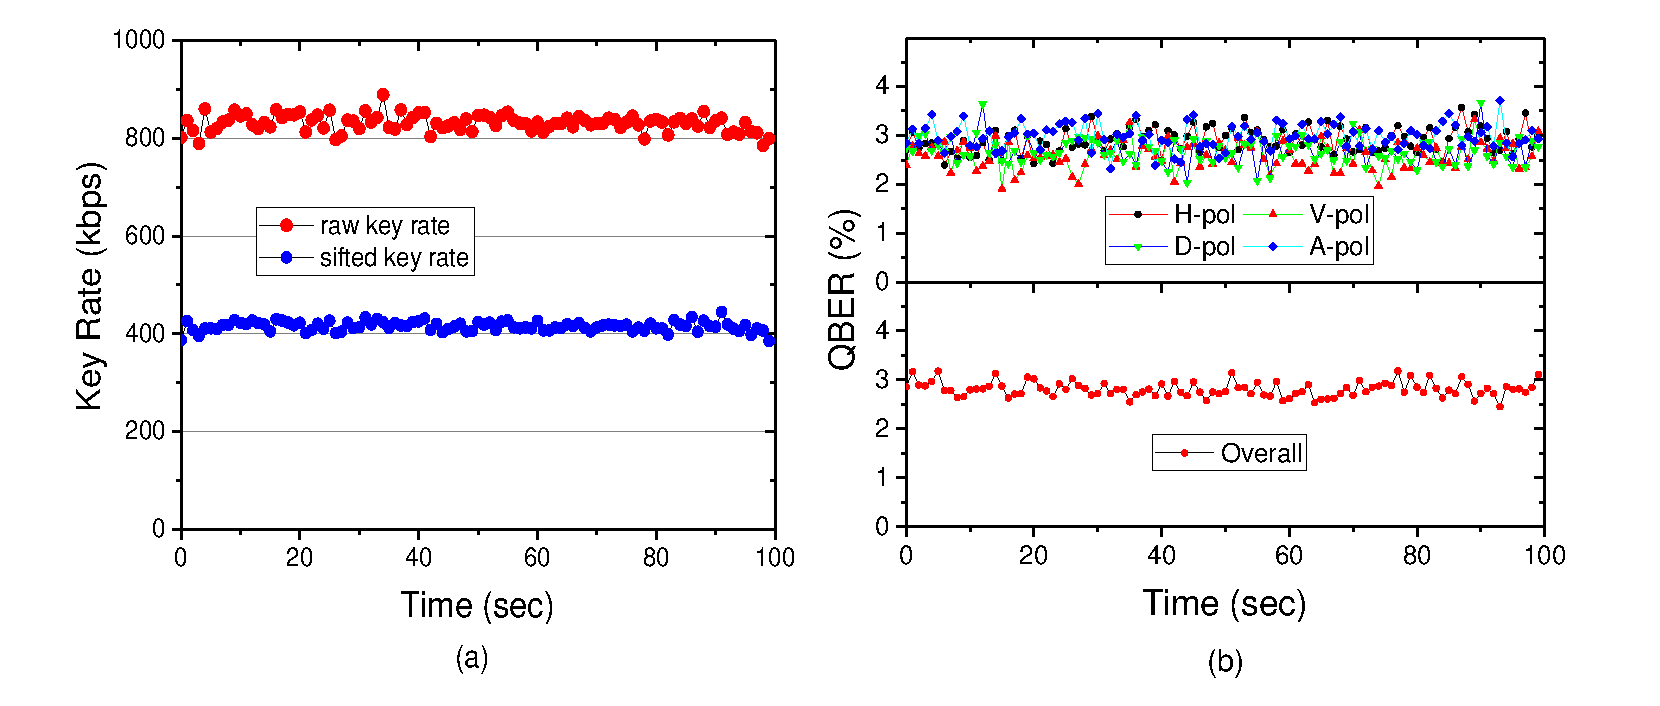
\includegraphics[height=5.6cm]{QKD_result}
  \caption{Test result for the PBS module in a free-space BB84 protocol test-bed at the clock rate of 100 MHz. (a) Raw key rate and sifted key rate for 100 sec and (b) QBER of four channels and overall QBER for 100 sec.}
  \label{fig:QKD_result}
\end{figure}
When bulk optic components were used instead of our PBS module, QBER and sifted key rate were measured to be 0.69\% and 1.56 Mbps, respectively.
The difference between the two cases is attributable to relatively high optical loss and low PER of our PBS module compared to the bulk optic components.
MZI-based PBS chips for 1.55 $\mu$m wavelength generally show better PER than the chip developed in this work \cite{Hashizume:2015ta}.
MZI works on the basis of phase relation that is determined by physical lengths of the two arms.
As the operation wavelength in this study is about half of that of optical telecommunication application, the performance of the MZI structure is more sensitive to small change in optical path length, and design optimization is more difficult.
Thus PER can be further improved by either optimizing the chip design with finer length variation or adopting smaller birefringence in BRW.


\section{Conclusion}
Waveguide-based integrated PBS module was developed for the first time that could separate the H/V/D/A polarizations for polarization-based BB84 QKD protocol in the 780 nm wavelength band.
The PBS module showed minimum PER of 17.6 dB.
When the module was tested in Bob part of a free-space QKD test-bed, the measured sifted key rate was 415 kbps and QBER was 2.81\% at clock rate of 100 MHz, respectively.


\section*{Funding}
This work was supported by Electronics and Telecommunications Research Institute (ETRI) grant funded by the Korean government. [Development of transceiver components and system control technologies for the polarization based free space quantum key distribution]
%\section*{Acknowledgments}
\end{document}
